% Dokumentklassen sættes til memoir.
% Manual: http://ctan.org/tex-archive/macros/latex/contrib/memoir/memman.pdf
\documentclass[a4paper,10pt]{article}
\usepackage{pdfpages}
\usepackage[a4paper]{geometry}
% Danske udtryk (fx figur og tabel) samt dansk orddeling og fonte med

% danske tegn. Hvis LaTeX brokker sig over æ, ø og å skal du udskifte
% "utf8" med "latin1" eller "applemac". 
\usepackage[utf8]{inputenc}
\usepackage[danish]{babel}
\usepackage[T1]{fontenc}
% \usepackage{setspace}
%\doublespacing
% Matematisk udtryk, fedes fymboler, theoremer og fancy ting (fx kædebrøker)
\usepackage{amsmath,amssymb}
\usepackage{bm}
\usepackage{amsthm}
\usepackage{tikz}
%\usepackage{mathtools}
% Kodelisting. Husk at læse manualen hvis du vil lave fancy ting.
% Manual: http://mirror.ctan.org/macros/latex/contrib/listings/listings.pdf
\usepackage{listings}
\usepackage{verbatim}
\usepackage{hyperref}

\usepackage[section]{placeins}

% Fancy ting med enheder og datatabeller. Læs manualen til pakken
% Manual: http://www.ctan.org/tex-archive/macros/latex/contrib/siunitx/siunitx.pdf
%\usepackage{siunitx}
% Indsættelse af grafik.
\usepackage{graphicx}
%\usepackage{bussproofs}
\usepackage{natbib}

\usepackage[font=small,labelfont=bf,labelsep=space]{caption}
\usepackage{siunitx}
\sisetup{output-exponent-marker=\ensuremath{\mathrm{E}}}
%Install abstract package and and \usepackage{abstract}
\renewcommand{\abstractname}{Abstract}    

% Reaktionsskemaer. Læs manualen for at se eksempler.
% Manual: http://www.ctan.org/tex-archive/macros/latex/contrib/mhchem/mhchem.pdf
%\usepackage[version=3]{mhchem}
\author{Christian Budde Christensen, 20103616\\Nicklas Pingel, 20102222\\Lukas Walther, 20107539}
\title{Advanced Data Structures}
\date{\today}
\begin{document}
\maketitle
\tableofcontents 
\clearpage
\section{Worst Case Analysis}
\subsection{Fibonacci Heap}
\subsubsection*{Make-heap}
For this our implementation just creates an empty heap, and is implemented as our constructor for our Fibonacci Heap. As we create no trees and no nodes this will yield a $O(1)$ running time.
\subsubsection*{Find-Min$(H)$}
By maintaining a pointer \texttt{minRoot}($\min(H)$) which points at the node with minimum key. The actual cost of this will be 1 for our structure. We do not change our number of trees($t(H)$ or mark any nodes($m(H)$). Because of this \texttt{FIND-MIN} will run in $O(1)$ time.
\subsubsection*{Insert$(H,x,k_k)$}
We add a tree with a single node to $H$ storing the item $x$ with our key $k_x$. We may also need to update our $\min(H)$. In this operation we increase our $t(H)$ by one but we don't mark any nodes. The cost will be adding a node, updating $\min(H)$, plus our increased $t(H)$. The combined cost will then be $2+1=O(1)$.
\subsubsection*{Meld$(H_1, H_2)$}
We combine $H1$ and $H2$ together, forming a new heap $H$. We update $\min(H)$ accordingly. For putting trees together we do not change either $t(H)$ nor $m(H)$. The total cost is then putting the trees together and setting $\min(H)$, $2+0=O(1)$.
\subsubsection*{Delete-Min$(H)$}
We create the array of pointers which has a cost $\leq$ max degree of any node in our Fibonacci heap($d_n$) + 1. Lets suppose we start with $k$ trees in our doubly linked list of roots, and perform $l$ link operations we then perform $k+l$ work, and end up with $k-l$ trees. The worst case for linking the heap would be $n$ elements in our doubly-linked list of roots, with none of these combined in a tree. $t(H)$ will be reduced by $k/2$, and we do not mark any nodes. The worst case is then $O(n)$. 

For the amortized case we look at the potential change, given as $\Delta_i \geq -2l$. The amortized cost, of the $i$-th operation with respect to the potential function is $\hat{c_i} = c_i + \Delta_i \leq 2(k - l) + d_n + 1$. But will be $k - l\leq d_n + 1$ because we can have at most one tree of each rank so, $\hat{c_i}\leq 3d_n + 3 = O(\log n)$.

\subsubsection*{Decrease-Key$(H, x, k_x)$}
We decrease the key of the node $x$ to the new key $k_x$, and if the heap property becomes violated, the node is cut from its parent. We also mark up the tree untill we hit a node or an unmarked node. For each cut we unmark a node when making the node a root.

We increase $t(H)$ by $k$, the number of cuts and in the end mark at most 1, so $m(H)$ increase at most 1. The overall cost is computed as $c_i=1+k=O(k)$ where each cut operation takes $O(1)$. This will in the worst case, where we have $\log n$ number of nodes we need to cut yield a worst case running time of $O(\log n)$.

When we look at the amortized running time, we first look at the potential drop
\begin{align*}
t(D_i)-t(D_{i-1}) &= 1 + k, m(D_i)-m(D_{i-1})\leq -k+1\\
\text{potential drop, } \Delta_i &= 2(t(D_i)-t(D_{i-1}))+3(m(D_i)-m(D_{i-1}))\\
&\leq 2(1+k)+3(-k+1)\\
&= -k+5
\end{align*}
Thus we can see that the amortized cost, $\hat{c_i}$, of \texttt{DECREASE-KEY} is
\begin{align*}
  \hat{c_i} &= c_i + \Delta_i\\
  &\leq (1+k)+(-k+5)\\
  &= 6 = O(1)
\end{align*}
\subsection*{Delete($H, x$)}
We delete by first decreasing the key of $x$ to the lowest value of our heap and then \texttt{DELETE-MIN} to remove it. The worst case is bounded by the worst case of \texttt{DECREASE-KEY} plus the worst case of \texttt{DELETE-MIN}. By combining these we get $O(\log n) + O(n) = O(n)$ in the worst case. \texttt{DELETE} is also bound by the method's amortized time, $\hat{c_i}$

\begin{align*}
\hat{c_i} =& \text{ amortized cost of Decrease-Key}\\
&+\text{amortized cost of Delete-Min}\\
=& O(1) + O(\log n)\\
=& O(\log n)
\end{align*}


\subsection{Binary Heap}
\subsubsection*{Make-heap}
As for Fibonacci Heap we only construct the heap, but we do not construct any nodes. Because of this we have $O(1)$ running time.

\subsubsection*{Find-Min$(H)$}
Because of the heap property, the minimum element will always be present at the root of the heap. Therefore the worst case is $O(1)$.

\subsubsection*{Insert$(H,x,k_x)$}
The worst case complexity for inserts will be having to insert in the case of inserting the yet smallest element into the tree of height $h$ as this would make us bubble up the tree all the way into root this would give a running time of $O(h)$.

The longest we can bubble up in a tree of size $n$ is $\log n$, making the worst case $O(\log n)$.
\subsubsection*{Delete-Min$(H)$}
We start by deleting the minimum, we place the last element in the hole created at the root. This will leave the heap property possibly violated at the root level. So we bubble down until the violation is stopped.

The longest we have to bubble down to stop the violation would be the entire depth of the tree, giving us $O(\log n)$ running time in the worst case.
\subsubsection*{Decrease-Key$(H, x, k_x)$}
Lowers the current value of the item $x$, to new priority value $k_x$. Now the heap property could possibly be violated for the parent and node $x$. So we need to bubble $x$ up until the violation is stopped.

The longest we have to bubble up to stop the violation would be the entire depth of the tree, giving us $O(\log n)$ running time in the worst case.
\subsubsection*{Delete($H, x$)}
First we use \texttt{DECREASE-KEY} to set the node $x$ to the lowest value, then we use \texttt{DELETE-MIN} to remove this node, because this is now the smallest.

The worst case for \texttt{DELETE} is bounded by the worst case for \texttt{DECREASE-KEY} + the worst case for \texttt{DELETE-MIN}. This will give us $O(\log n) + O(\log n) = O(\log n)$ in the worst case.

\begin{table}
  \begin{center}
    \begin{tabular}{l|c|c}
      & Fibonacci Heap & Binary Heap \\
      \hline
      Make-Heap    & $O(1)$             & $O(1)$\\
      Find-Min     & $O(1)$             & $O(1)$\\
      Insert       & $O(1)$             & $O(\log n)$\\
      Meld         & $O(1)$             & NA\\
      Delete-Min   & $O(n)$             & $O(\log n)$\\
      Decrease-Key & $O(\log n)$        & $O(\log n)$\\
      Delete       & $O(n)$             & $O(\log n)$
    \end{tabular}
    \caption{Worst case execution time for Fibonacci and Binary Heap}
  \end{center}
\end{table}
\section{Heap Experiments}
All experiments were run on a linux machine, using an Intel Xeon W3520 running at 2.67GHz. The computer is equipped with 24 GB of RAM of type DDR3. Experiments did not require more than 10 gigabyte of memory, so it is safe to assume that the swap would not be used by our programs. The processor has four physical cores, one of which was dedicated to running our experiments, so influence of other programs should be very small.

All experiments were timed with the \texttt{clock\_gettime} method from the c++ standard library, which offers resolutions close to a few nanoseconds. The \texttt{CLOCK\_PROCESS\_CPUTIME\_ID} flag is used, which measures the CPU-time spent on running the program, instead of using real-world time, which could potentially be inflated by background processes.
All experiments write their results to different files. Care is taken to only measure the time spent computing the methods under observation, not the writing to files or generation of input or graphs.

\section{Implementation}
Fibonacci heaps are implemented very much like in Introduction to Algorithms [CLRS] chapter 19. Fibonacci Heap's nodes are arranged in doubly linked circular lists, where each node has a pointer to its parent, one child, and the nodes left and right to it. There are no relevant differences in our implementation, compared to Fredman and Tarjans or CLRS version, other than that we use a more object-orientated style of programming.

Binary heaps are implemented with a pointer-based datastructure, instead of organizing the nodes implicitly within an array. This means, to find the last node correctly, of find out where to insert a new node, without using $O(n)$ time, we use decimal to binary conversion to compute a path trough the heap to the position that is needed. This can be achieved in $O(\log(n))$ time, without changing the established asymptotic running time. We chose to use a pointer-based structure, to make the heaps more comparable to each other.%% As we will show later, when the different heap's methods have the same asymptotic behaviour, they also achieve the same measured running time %%

\subsection{Fibonacci Heap}
\subsubsection{Insert$(H,x,k_x)$}
{\bf Hypothesis}\\
We have that \texttt{FIBONACCI-HEAP-INSERT} performs in $O(1)$ time. This means that when we perform $N$ insertions into a fibonacci-heap we expect to measure a running time that increases linearly with the number of insertions, yielding a running time of $O(N)$ for $N$ insertions.\\
The experiment consists of inserting $N$ elements into the heap. The element's keys range from $2N$ to $N$, which has no effect on the execution time of \texttt{FIBONACCI\--HEAP\--INSERT}, but is usefull for later experimentation with \texttt{FIBONACCI\--HEAP\--DECREASE\--KEY}.\\
Below we present the measured running times for \texttt{FIBONACCI\--HEAP\--INSERT} for $N$ elements.\\\\
{\bf Results}
\begin{table}
  \begin{center}
    \begin{tabular}{l|r|r}
      $N$ & measured insert time(s) & measured insert/N time(s)\\
      \hline
      10       & \num{5.971E-7}     & \num{5.971E-8}\\
      100      & \num{3.424E-6}     & \num{3.424E-8}\\
      1000     & \num{4.215E-5}     & \num{4.215E-8}\\
      10000    & \num{5.587E-4}     & \num{5.588E-8}\\
      100000   & \num{0.0056}       & \num{5.668E-8}\\
      1000000  & \num{0.0610}       & \num{6.100E-8}\\
      10000000 & \num{0.6070}       & \num{6.070E-8}
    \end{tabular}
    \caption{Bounds and measured running time}
  \end{center}
\end{table}\\\\
{\bf Conclusion}\\
The time spent per single insert operation hovers around a constant factor. Even though the numbers do not form a horizontal line on the graph, they are in the same order of magnitude, excluding the possibility of an exponential growth. The second graph gives a good impression of \texttt{FIBONACCI-HEAP-INSERT} running in constant time for a single element, as the number of elements to be inserted tenfold, the running time also tenfolds. Thus we can safely assume that the \texttt{FIBONACCI-HEAP-INSERT} method actually runs in constant time.

\subsubsection{Decrease-Key$(H,x,k_x)$}
{\bf Hypothesis}\\
The amortized running time for \texttt{FIBONACCI-HEAP-DECREASE-KEY} is $O(1)$ and the worst case running time is $O(\log n)$. The experiment consists of a heap with $N$ elements with increasing keys from $N$ to $2N$, where \texttt{FIBONACCI-HEAP-DECREASE-KEY} is called with elements in decreasing order of their key, reducing their key by $N$, which means that the heap updates it's minimum element with each call. The expectation is, that after some calls to \texttt{FIBONACCI-HEAP-DECREASE-KEY}, the cost of calling \texttt{FIBONACCI-HEAP-DECREASE-KEY} will approach a constant, which implies that $N$ calls to \texttt{FIBONACCI-HEAP-DECREASE-KEY} will have an amortited running time of $O(N)$.\\\\
{\bf Results}
\begin{table}
  \begin{center}
    \begin{tabular}{l|r|r}
      $N$ & measured decrease time(s) & measured decrease time(s) /N \\
      \hline
      10       & \num{5.492E-7}     & \num{5.492E-8}\\
      100      & \num{3.590E-6}     & \num{3.589E-8}\\
      1000     & \num{3.244E-5}     & \num{3.245E-8}\\
      10000    & \num{3.195E-4}     & \num{3.200E-8}\\
      100000   & \num{0.0034}       & \num{3.434E-8}\\
      1000000  & \num{0.0372}       & \num{3.718E-8}\\
      10000000 & \num{0.3847}       & \num{3.847E-8}
    \end{tabular}
    \caption{Bounds and measured running time}
  \end{center}
\end{table}\\\\
{\bf Conclusion}\\
The measurement divided by the number of \texttt{FIBONACCI-HEAP-DECREASE-KEY} calls approach a factor of \num{3.786E-8}, within a small margin of error, when we ignore the first measurement of size 10, as this is easily inflated due to its very short running time. We can safely conclude that the cost of each \texttt{FIBONACCI-HEAP-DECREASE-KEY} call converges to a constant factor, after a number of calls to the method, though one could still take measurements to find after how many calls in succession \texttt{FIBONACCI-HEAP-DECREASE-KEY} comes close to constant running time.

\subsubsection{Delete-Min$(H)$}
{\bf Hypothesis}\\
The worst case running time for \texttt{FIBONACCI-HEAP-DELETE-MIN} is $O(n)$ and the amortized running time is $O(\log n)$. In this experiment, we start out with a heap of size $N$ and call \texttt{FIBONACCI-HEAP-DELETE-MIN} until the heap is empty. For this amount of delete-min operations, the total running time is expected to be $O(\log(N!))$. Due to the amortized running time, we expect $N$ \texttt{FIBONACCI-HEAP-DELETE-MIN} operations to perform much better than \[G(N) = \sum^N_{n=1} n = \frac{N(N-1)}{2}.\]\\\\
{\bf Results}\\
\begin{table}
  \begin{center}
    \begin{tabular}{l|r|r|r}
      $N$ & expected running time(s) & measured running time(s) & $G(N)$\\
      \hline
      10       & \num{20}           & \num{1.981E-6} & \num{45}\\ 
      100      & \num{522}          & \num{2.523E-5} & \num{4950}\\
      1000     & \num{8504}         & \num{0.000254} & \num{499500}\\
      10000    & \num{118261}       & \num{0.00383}  & \num{49995000}\\
      100000   & \num{1516460}      & \num{0.04043}  & \num{5E+9}\\
      1000000  & \num{18488855}     & \num{0.43195}  & \num{5E+11}\\
      10000000 & \num{218107833}    & \num{3.71978}  & \num{5E+13}
    \end{tabular}
    \caption{Bounds and measured running time}
  \end{center}
\end{table}\\\\
{\bf Conclusion}\\
The measured running times show that the running time increases at most at the same rate as the theoretical bound we expected and increases not at all like the worst-case bound for $N$ insertions. We can conclude that this implementation of \texttt{FIBONACCI-HEAP-DELETE-MIN} operates in the expected amortized bound of $O(\log n)$.

\subsection{Binary Heap}
\subsubsection{Insert$(H,x,k_x)$}
In this section will we explore the running time of Binary-Heaps insert method. The running time is analyzed in two different ways. At first, we run a number of inserts accumulative and observe the total running time of $N$ \texttt{BINARY-HEAP-INSERT} operations. Then we analyze \texttt{BINARY-HEAP-INSERT} operations relative to the height of the heap.\\\\
{\bf Hypothesis}\\
To measure the running time, $N=10^k$ elements with decreasing key are inserted into the heap in succession to achieve worst-case behaviour. This is done 50 times to compute an average. Because the \texttt{BINARY-HEAP-INSERT} operation is done $N$ times in succession, we expect the running time to be the sum over the individual insert operation at any given size of the heap, which is called $n$.
Thus, we expect to measure a running time of the form: \[\sum^N_{n=1}\log n.\]
We have $\log(a)+\log(b)=\log(a\cdot b)$ so 
\begin{align*}
  f(N)=\sum^N_{n=1}\log(n)&=\log(1)+\log(2)+\cdots+\log(N)\\
  &=\log(1\cdot2\cdot3\cdots N)\\
  &=\log(N!)
\end{align*}

The numbers for $f(N)$ in the graph section are only approximate, as computing the faculty of numbers bigger than 100 is troublesome. 

In the second experiment, an emtpy heap is used, and elements are inserted layer by layer. To increase the height of the heap by one every time, we insert $2^k$ elements, where k is the height of the heap. Each element is inserted with a key that is smaller than the smallest key currently in the heap, which means that the element has to travel through the $k$ layers in the heap to reach the top. This is the worst case scenario for \texttt{BINARY-HEAP-INSERT}.

For each layer, we measure the time for running \texttt{BINARY-HEAP-INSERT} $2^k$ times and divide the running time by the numbers of elements inserted, which yields an average running time for the current height of the graph.

We also count the number of comparisons made for each size, which we expect to be the logarithm of the height of the heap and time single inserts at the same height 50 times to compute an average time per insertion at the given size.\\\\
{\bf Results}\\
In the table below, we present the measured running times, and the computed function $f(N)$.
\begin{table}
  \begin{center}
    \begin{tabular}{l|r|r}
      $N$ & $f(N)$ & measured running time(s) \\
      \hline
      10       & 20         & \num{1.6487E-6}\\
      100      & 522        & \num{2.3691E-5}\\
      1000     & 8504       & \num{2.6033E-4}\\
      10000    & 118261     & \num{3.4728E-3}\\
      100000   & 1516460    & \num{4.1341E-2}\\
      1000000  & 18488855   & \num{0.4934}\\
      10000000 & 218107833  & \num{5.5171}
    \end{tabular}
    \caption{Bounds and measured running time}
  \end{center}
\end{table}
\begin{table}
  \begin{center}
    \begin{tabular}{l|r|r}
      size & number of comparisons & time per comparison\\
      \hline
      10       & 3  & \num{4.556E-7}\\
      100      & 6  & \num{4.507E-7}\\
      1000     & 9  & \num{4.514E-6}\\
      10000    & 13 & \num{6.597E-7}\\
      100000   & 16 & \num{7.105E-7}\\
      1000000  & 19 & \num{1.907E-5}\\
      10000000 & 23 & \num{1.081E-6}
    \end{tabular}
    \caption{Bounds and measured running time}
  \end{center}
\end{table}\\\\
{\bf Conclusion}\\
If we plot the graph for the proposed function and the measured running time on a doubly logarithmic graph, then we see they have the same tendency. We can safely discard the measured running times for 10 elements, as running times this close to single microseconds may easiliy be inflated. We observe that the running time increase at the same rate as the theoretical bound, this means that our measured running time conforms to the expected running time $O(\log N!)$. Hereby the running time of binary heap's insert conforms to the expected asymptotic running time $O(\log n)$.

As expected, the number of comparisons for an insert operation is logarithmic in the size of the heap. Comparing the running times for insertion divided by the number of comparisons shows some irregularities. At heap size of 10, 100, 10.000, 100.000 and 10.000.000 are close to the same constant, the values for heap sizes of 1.000 and 1.000.000 vary wildly. This can possibly be explained by the elements being compared sometimes being on few pages of memory, whilst other times being spread amongst multiple pages of memory, though we have no further data to back up this claim.
\subsubsection{Decrease-Key$(H,x,k_x)$}
{\bf Hypothesis}\\
The \texttt{BINARY\--HEAP\--DECREASE\--KEY} method has a worst case running time of $O(\log n)$ where $n$ is the current size of the heap. This means, when we run \texttt{BINARY\--HEAP\--DECREASE\--KEY} on every element, the asymptotic running is expected to be $O(n\log n)$ in the worst case. Our experiment consists of a Binary Heap where $N$ elements were inserted with decreasing keys from $2N$ to $N+1$ and we measure the time it takes to call \texttt{BINARY\--HEAP\--DECREASE\--KEY} on every element once. We start with the element with the biggest key, $2N$, and decrease its key to $N$. This gives us the worst case for the \texttt{BINARY\--HEAP\--DECREASE\--KEY} methods, as $N$ is the smallest key at this point. We repeat this process for the next biggest element, which has key $2N-1$ and decrease its key to $N-1$, again giving rise to the worst case scenario. We repeat this process for all remaining elements, decreasing the key of the element with key $2N-i$ to $N-i$. As we repeat this process for $N$ elements, the total running time for $N$ \texttt{BINARY\--HEAP\--DECREASE\--KEY} operations is $O(N\log N)$.

In the table below, we present the measured running times, and the function $O(N\log N)$.
{\bf Results}
\begin{table}
  \begin{center}
    \begin{tabular}{l|r|r}
      $N$ & $O(N\log N)$ & measured running time(s)\\
      \hline
      10       & 33         & \num{7.506E-7}\\
      100      & 644        & \num{1.0843E-5}\\
      1000     & 9966       & \num{0.000141}\\
      10000    & 132877     & \num{0.001805}\\
      100000   & 1660964    & \num{0.0242}\\
      1000000  & 19931569   & \num{0.3163}\\
      10000000 & 232534967  & \num{3.7488}
    \end{tabular}
    \caption{Bounds and measured running time}
  \end{center}
\end{table}\\\\
{\bf Conclusion}\\
Observe that the graph shows the same inclination for the measured data and the $n\log n$ function. The measured running time increases proportionally just as much as the $n\log n$ theoretical bound, thereby a single \texttt{BINARY\--HEAP\--DECREASE\--KEY} performs in $O(\log n)$ time.

\subsubsection{Delete Min$(H)$}
{\bf Hypothesis}
The \texttt{BINARY\--HEAP\--DELETE\--MIN} method has a worst case running time of $O(\log n)$ where $n$ is the current size of the heap. If we call \texttt{BINARY\--HEAP\--DELETE\--MIN} as many times as there are elements in the heap, we would have a running of $O(\log N!)$, exactly like \texttt{BINARY\--HEAP\--INSERT}. The experiment consists of calling \texttt{BINARY\--HEAP\--DELETE\--MIN} until the heap of size $N$ is empty.

In the table below, we present the measured running times, and the function $O(N\log N)$. The second table shows the running times for insertion divided by the running times for deletion.\\\\
{\bf Results}\\
\begin{table}
  \begin{center}
    \begin{tabular}{l|r|r}
      $N$ & $O(N\log N)$ & measured running time(s)\\
      \hline
      10       & 33         & \num{1.8486E-6}\\
      100      & 644        & \num{2.3476E-5}\\
      1000     & 9966       & \num{2.8870E-4}\\
      10000    & 132877     & \num{3.4556E-3}\\
      100000   & 1660964    & \num{0.0410}\\
      1000000  & 19931569   & \num{0.4842}\\
      10000000 & 232534967  & \num{5.7055}
    \end{tabular}
    \caption{Bounds and measured running time}
  \end{center}
\end{table}
\begin{table}
  \begin{center}
    \begin{tabular}{l|r}
      $N$ & $\dfrac{\text{insert}}{\text{delete}}$\\
      \hline
      10       & \num{0.89}\\
      100      & \num{1.01}\\
      1000     & \num{0.90}\\
      10000    & \num{1.00}\\
      100000   & \num{1.01}\\
      1000000  & \num{1.02}\\
      10000000 & \num{0.97}
    \end{tabular}
    \caption{Bounds and measured running time}
  \end{center}
\end{table}
{\bf Conclusion}\\
Observe that the measurements for \texttt{BINARY-HEAP-DELETE-MIN} increase at most as fast as the theoretical bound, but also are very close to the measured running times of \texttt{BINARY-HEAP-INSERT}. When we divide the running time of \texttt{BINARY-HEAP-INSERT} with the runnning time of \\\texttt{BINARY\--HEAP\--DELETE\--MIN} for every given size, we find that the average factor is 0.97 within a small margin of error. We can conclude that the running time for deletion increases at the same rate as those for insertion, which gives us that our implementation of \texttt{BINARY-HEAP-DELETE-MIN} performs within $O(\log n)$ bounds, just like insertion.

\subsection{Comparison}
Comparing the operations for Binary Heap and Fibonacci Heap shows that insertions are always faster in Fibonacci Heaps, as these can be performed in constant time opposed to the logarithmic worst time performance for binary heaps. Also when purely calling \texttt{DECREASE\--KEY} many times in a row, a Fibonacci Heap performs better and better compared to a Binary Heap, the bigger the heap is. Only the \texttt{DELETE\--MIN} methods perform comparable with about a factor of one, until heap sizes of 10.000.000 are used, where Fibonacci Heaps starts to perform slightly faster.

\section{Dijkstra}
For experiments with the \texttt{DIJKSTRA} algorithm, we use three different kinds of graphs, each giving rise to a different number of \texttt{DECREASE\--KEY} calls.
\subsection{Complete Directed Graph}
The complete graphs used here, closely resemble K-graphs, but are not bi-directionally connected. A complete graph of size $N$ consists of $N$ nodes and $N(N-1)/2$ edges and is build in the following way. The nodes are indexed from 0 to $N-1$, where node 0 is our source node for the \texttt{DIJKSTRA} algorithm. Each node $i$ is connected to its successor $i+1$, with an edge of weight 1, and to all other nodes $i+2$ to $N-1$ with weight $2N+1-i$. This graph is designed in such a way that the number of decrease key calls is equal to the number of edges, giving rise to an exponential amount of calls.

\subsection{Random Graphs}
Random graphs are characterized by their size $N$ and density $D$, having $N$ nodes and each node having $D$ directed edges from it. Random graphs are generated by creating $N$ edges, and for every node choosing $D$ seperate other nodes and connecting to them with a random weight. The number of decrease key calls for a graph of a given size grows with the density of the graph, but increasing the density yields a diminishing return on the number of \texttt{DECREASE\--KEY} calls. 

On the table below are the number of decrease key calls when running dijkstra on a graph of size 6250 and different densities in percent.

\begin{table}
  \begin{center}
    \begin{tabular}{l|r}
      density & number of \texttt{DECREASE\--KEY} \\
      \hline
      0.01 & 20654\\
      0.11 & 37079\\
      0.21 & 41108\\
      0.31 & 43762\\
      0.41 & 45930\\
      0.51 & 47363\\
      0.61 & 48292\\
      0.71 & 47966\\
      0.81 & 50356\\
      0.91 & 50833
    \end{tabular}
    \caption{Decrease-Key calls for graph of size 6250 and different densities.}
  \end{center}
\end{table}

\subsection{Linear Graphs}
These simple graphs consist of $N$ nodes and to special nodes, the source and the sink. The source is simply connected to the $N$ nodes with increasing weights from 1 to $N$. Each node $i$ of the $N$ nodes is then connected to the sink with a weight of $N\cdot 2 +1 - i\cdot 2$. This results in $2N$ calls to decrease key. $N$ calls for the $N$ nodes connected from the source. And one call for each of the $N$ nodes, because the total weight from the source to the sink is $2N +1 -i$ at that point, where $i$ increases by one with each node visited.

\section{Dijkstra Experiments}

\subsection*{Hypothesis}
In the following tests we wish to cover the running time for the implementation of \texttt{FIBONACCI\--HEAP\--DECREASE\--KEY} with graphs of increasing sizes against \texttt{BINARY\--HEAP\--DECREASE\--KEY}. We first run \texttt{DIJKSTRA} using the Fibonaci Heap implementation on graphs with increasing sizes, then we do the same for the Binary Heap implementation. The graphs we use are the three types of graphs explained above. We expect to see that the factor of increase for the running time will grow significantly slower for the Fibonacci Heap implementation than the Binary Heap implementation due to the amortized  \texttt{DECREASE-KEY} function. Furthermore we expect to find the shortest path in graphs yielding many \texttt{DECREASE-KEY} operations to be generally faster, when using Fibonacci Heaps instead of Binary Heaps. This is due to the cost of \texttt{DECREASE-KEY} beeing significantly lower in the Fibonacci Heap implementation than in the Binary Heap implementation which has been shown in previous tests.

According to Introduction to Algorithms [CLRS] page 662, the dijkstra algorithm has an asymptotic running time of $O((V+E)\log V)$ when using a binary heap and $O(E + V\log V)$, where $V$ is the number of vertices in the graph and $E$ the number of edges. Assuming one can achieve worst-case behaviour with certain types of graphs, the difference in measured running time should be significant. Given that our implementations of the heaps have similar running times for deletion, only the running times of insertion and decrase key operations will make a difference in the total running time of dijkstras algorithm. Also the contribution of insertions to the running time should be less significant, when the number of decrease key calls is exponential to the number of vertices. 
\subsection*{Results}

\begin{table}
  \begin{center}
    \begin{tabular}{l|l}
      size & Binary time(s)/ Fibonacci time(s) \\
      \hline
      10    & 0.8860\\
      20    & 1.2114\\
      40    & 1.2028\\
      80    & 1.2640\\
      160   & 1.2664\\
      320   & 1.4182\\
      640   & 1.4059\\
      1280  & 1.3662\\
      2560  & 1.4957\\
      5120  & 1.4357\\
      10240 & 1.5449
    \end{tabular}
    \caption{Increasing factor Binary running time divided by Fibonacci running time on Dijkstra on linear graphs}
  \end{center}
\end{table}

The factor we see in the table 11 is increasing even though slowly. Fibonacci Heap continously gets faster than Binary Heap for increasing size of graphs. This increase is not very significant and can be attributed to the constant factors adding up. This is due to this kind of graphs resulting in a heap, where decrease key calls do only make a single comparison. These linear graphs are very sparse, having only two edges for every node, which also limits the number of \texttt{DECREASE\--KEY} calls to two times the number of vertices.

\begin{table}
  \begin{center}
    \begin{tabular}{l|l}
      size & Binary time(s)/ Fibonacci time(s) \\
      \hline
      10    & 0.9342700643\\
      20    & 1.2397301177\\
      40    & 1.2355809946\\
      80    & 1.3722459278\\
      160   & 1.0779121349\\
      320   & 1.2237703573\\
      640   & 1.2577482582\\
      1280  & 1.1286911763\\
      2560  & 1.1743038137\\
      5120  & 1.1949918895\\
      10240 & 1.1898308224
    \end{tabular}
    \caption{Running times of Dijkstra with Binary Heaps divided by running time with fibonacci heap.}
  \end{center}
\end{table}

The ratio of dijkstras running times with a binary heap divided by running times using a fibonacci heap is shown in table 12. This ratio stays mostly above one, meaning that the fibonacci heap implementation performs faster, when running dijkstra on k-graphs. These graph feature an exponential amount of decrease key operations, with graphs of size 10240 calling \texttt{DECREASE\--KEY} more than fifty million times. The number of \texttt{DECREASE\--KEY} calls is also equal to the number of edges in the graph. 

\begin{table}
  \begin{center}
    \begin{tabular}{l|l|l}
      density & Binary time(s)/ Fibonacci time(s) & average nmumber of decrease-key calls \\
      \hline
      0.001 & 1.0239 & 20259.1\\
      0.051	& 0.9737 & 59818.9\\
      0.101	& 1.0044 & 66949.4\\
      0.151	& 0.9691 & 70712.6\\
      0.201	& 0.9932 & 73892.5\\
      0.251	& 0.9836 & 76003.9\\
      0.301	& 0.9859 & 77785.9\\
      0.351	& 0.9916 & 79585.1\\
      0.401	& 0.9864 & 80936.8\\
      0.451	& 0.9873 & 81876.1\\
      0.501	& 0.9904 & 82986.9\\
      0.551	& 0.9752 & 84102.8\\
      0.601	& 0.9753 & 85045.8\\
      0.651	& 0.9745 & 85692.9\\
      0.701	& 0.9897 & 86514.9\\
      0.751	& 0.9905 & 87129.7\\
      0.801	& 0.9751 & 87848.2\\
      0.851	& 0.9911 & 88383.9\\
      0.901	& 0.9899 & 89157  \\
      0.951	& 0.9899 & 89703.1\\
      1		& 0.9785 & 90267.3
    \end{tabular}
    \caption{Random graph with 10240 vertices. Comparison between Fibonacci and Binary running time for random graphs.}
  \end{center}
\end{table}
In table 13 we see that for different densities of random graphs with 10240 vertices, the difference between the running times are relatively small, with the binary heap implementaion performing slightly faster. Random graphs behave very differently, compared to the constructed graphs we used earlier. The number of \texttt{DECREASE\--KEY} calls increases slower and slower with increasing connectivity, while the number of edges in the graph approaches the number of vertices squared at a density of 100\%.

\subsection*{Conclusion}

Our implementations of binary heap and fibonacci heap do not give rise to hugely different running times for the presented types of graphs, altough using fibonacci heaps is slightly faster when the number of decrease key calls is close to the number of edges is the graph, as seen in the experiments with k-graphs.

We have not managed to achieve worst case behaviour for binary heaps decrease key calls with these graphs. In theory, binary heaps should perform worse when many decrease key operations are required, and those decrease key operations use the maximum number of comparisons.

We must conclude, according to our experiments, that the expected differences in running time have not manifested themselves when running dijkstra on these types of graphs. There may be other kinds of graphs, where the differences are more obvious, but we have not found them.
\clearpage
\appendix 
\section{Graphs}
\begin{figure}[h]
    \label{timeinsertfib}
  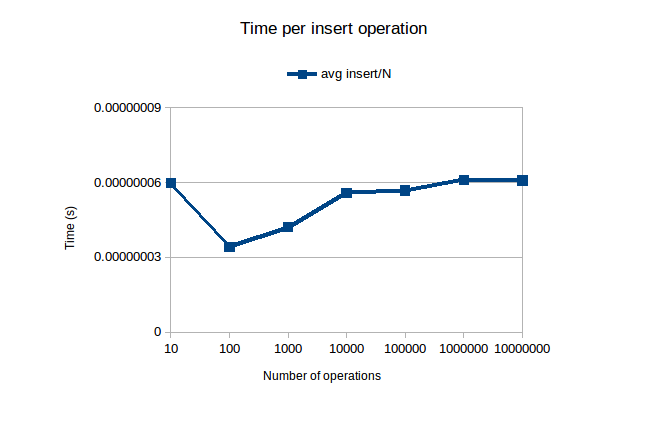
\includegraphics[width=15cm]{Time_per_insert_fibonacci.png}
  \caption{Time per insert operation in Fibonacci Heap}
\end{figure}

\begin{figure}[h]
    \label{timeprlayerbin}
  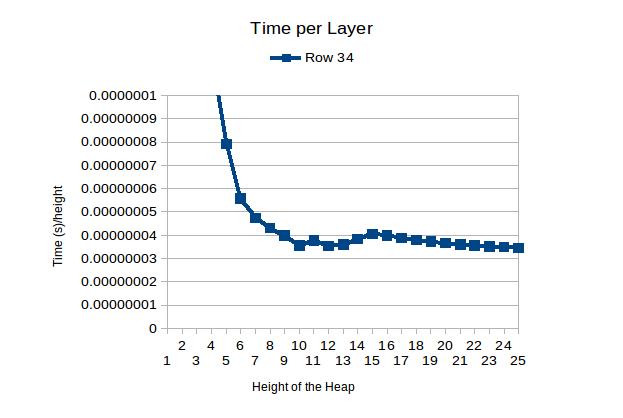
\includegraphics[width=15cm]{Time_per_layer_binary.png}
  \caption{Time per layer in Binary Heap}
\end{figure}

\begin{figure}[h]
    \label{timepercompbin}
  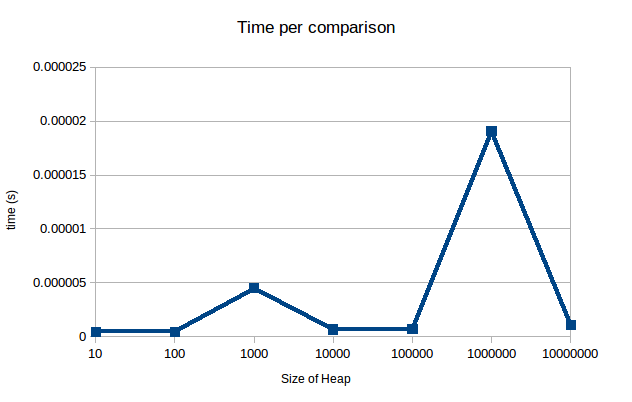
\includegraphics[width=15cm]{Time_per_comparison_binary.png}
  \caption{Time per comparison in Binary Heap}
\end{figure}

\begin{figure}[h]
    \label{timeinscomp}
  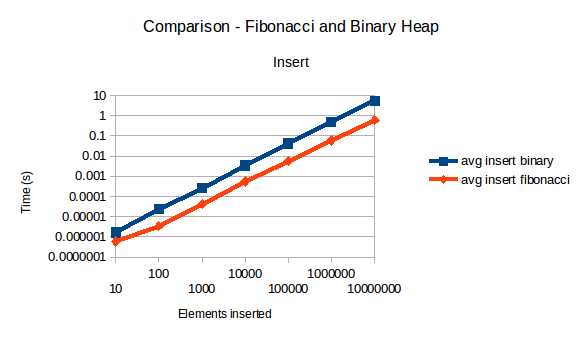
\includegraphics[width=15cm]{Time_insertion_comparison.png}
  \caption{Comparing insertions, Fibonacci against Binary heap}
\end{figure}

\begin{figure}[h]
    \label{deckeyboundbin}
  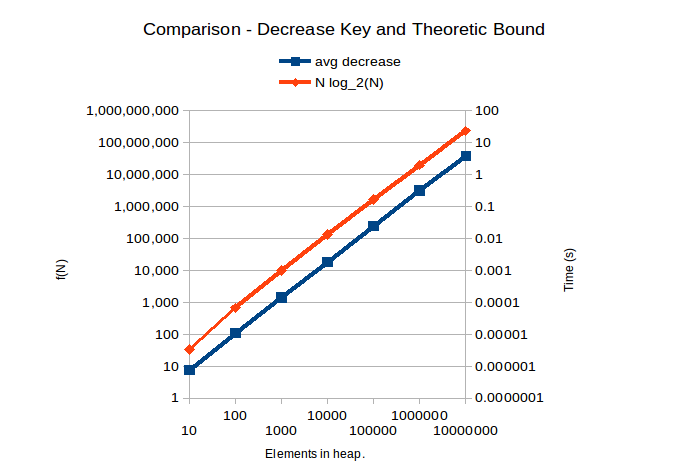
\includegraphics[width=15cm]{Decrease_key_bound_binary.png}
  \caption{Decrease key compared against theretic bounds in Binary heaps}
\end{figure}

\begin{figure}[h]
    \label{deckeyperelmfib}
  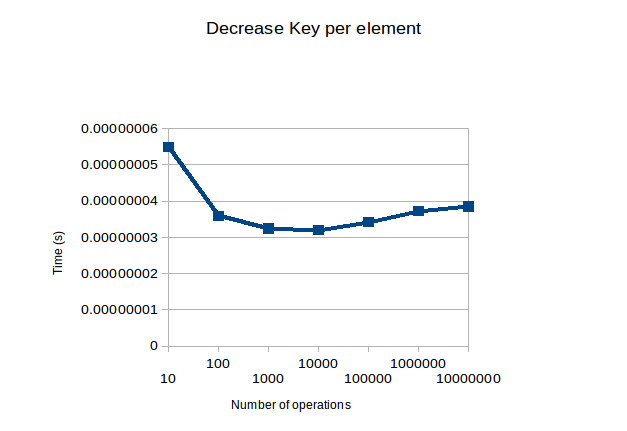
\includegraphics[width=15cm]{Decrease_key_per_element_fibonacci.png}
  \caption{Decrease key per element in Fibonacci Heaps}
\end{figure}

\begin{figure}[h]
    \label{delboundbin}
  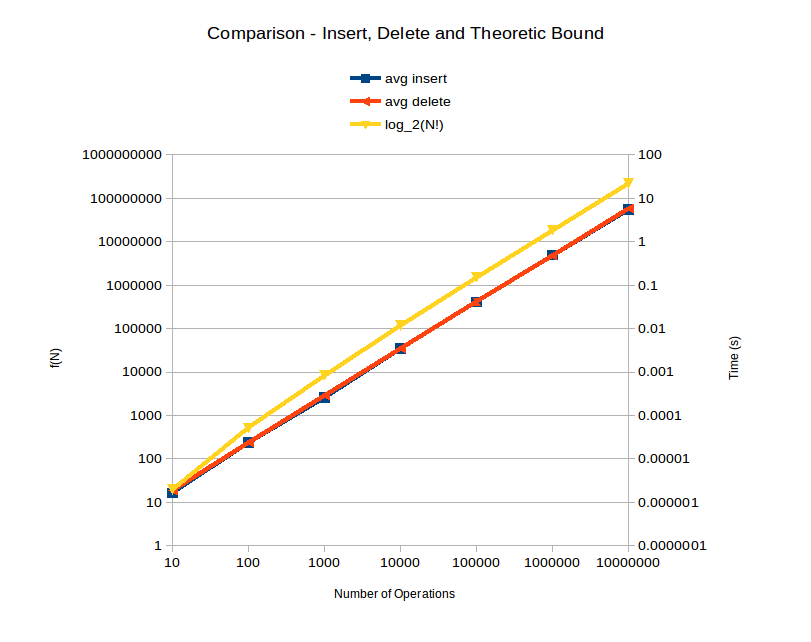
\includegraphics[width=15cm]{Delete_bound_binary.png}
  \caption{Comparing insertions, deletions against theretic boudns in Binary heap}
\end{figure}

\begin{figure}[h]
    \label{delboundfib}
  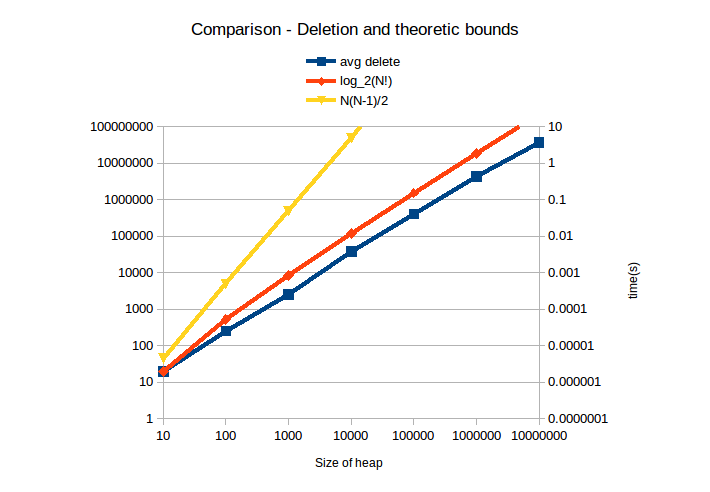
\includegraphics[width=15cm]{Delete_bound_fibonacci.png}
  \caption{Comparing deletions against theoretic bounds in Fibonacci Heaps}
\end{figure}

\begin{figure}[h]
    \label{instheoreticboundbin}
  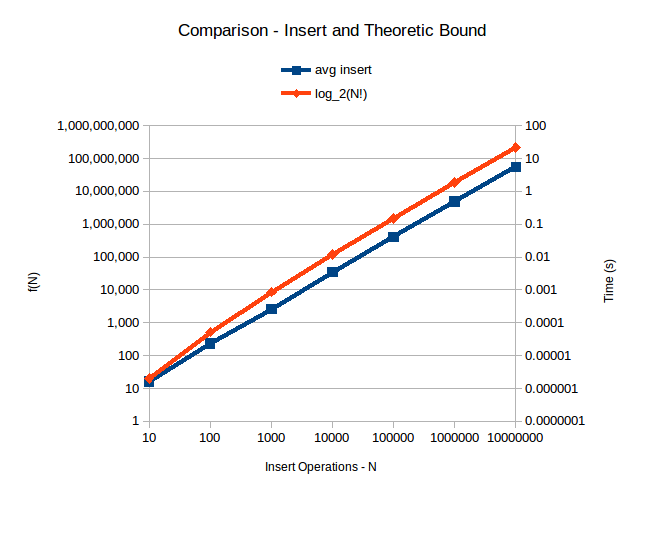
\includegraphics[width=15cm]{Insert_theoretic_bound_binary.png}
  \caption{Comparing insert operations and theoretic bound in Binary Heaps}
\end{figure}

\begin{figure}[h]
    \label{instheoreticboundfib}
  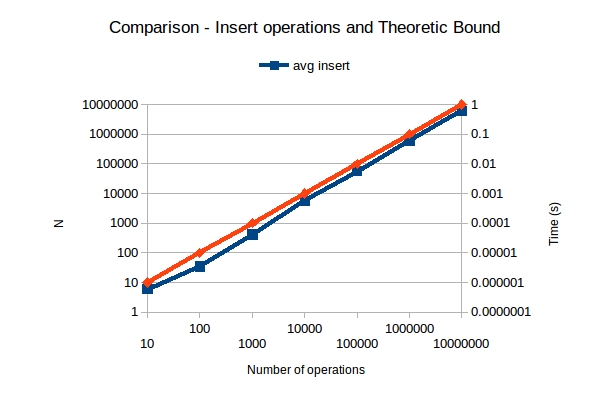
\includegraphics[width=15cm]{Insert_theoretic_bound_fibonacci.png}
  \caption{Comparing insert operations and theoretic bound in Fibonacci Heaps}
\end{figure}

\begin{figure}[h]
    \label{timeinsbin}
  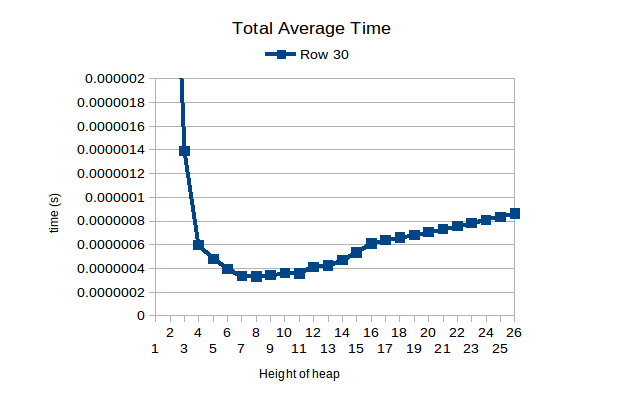
\includegraphics[width=15cm]{Total_time_binary.png}
  \caption{Time of running Binary Heap's insert method on a heap of given height.}
\end{figure}



\end{document}
